\chapter{DISEÑO EXPERIMENTAL Y RESULTADOS SOBRE EL ELLIPTIC DATASET}

Este capítulo traslada los fundamentos del Capítulo 3 a un entorno experimental concreto sobre el \textit{Elliptic Dataset}, el conjunto de transacciones reales de Bitcoin que sirve de referencia en la detección de actividad ilícita. El capítulo describe primero el preprocesamiento y una característica estructural del grafo que condiciona todo el estudio, a saber su dispersión extrema, y luego presenta el espacio factorial de configuraciones que se evaluó. A continuación se reportan el rendimiento predictivo y un fenómeno central del dominio, el colapso del desempeño entre la partición de validación y la de test, que obliga a estudiar la estabilidad de las explicaciones sobre validación. Finalmente, el capítulo documenta una corrección metodológica en la forma de generar las explicaciones que reordena el ranking de estabilidad entre arquitecturas y que constituye una de las contribuciones centrales de la tesis.

\section{Preprocesamiento y Análisis Exploratorio}

\subsection{Composición y Estructura Temporal del Conjunto de Datos}

El \textit{Elliptic Dataset} está compuesto por 203.769 nodos que representan transacciones de Bitcoin y 234.355 aristas que codifican el flujo de fondos entre ellas, con 166 features por nodo distribuidas a lo largo de 49 pasos temporales \cite{Weber2019Anti-MoneyForensics}. De esos nodos, únicamente 46.564 poseen etiqueta conocida, repartidos en 4.545 transacciones ilícitas y 42.019 lícitas, mientras que los 157.205 restantes permanecen sin clasificar. La clase ilícita representa así apenas el dos coma dos por ciento del total de nodos y establece una razón cercana a 1:9 respecto de la clase lícita dentro del subconjunto etiquetado, una proporción que ya de por sí refleja el desbalance característico del dominio AML y que los escenarios experimentales acentúan de forma deliberada. La Tabla \ref{tab:composicion} resume esta composición y fija las magnitudes sobre las que se construye el diseño experimental.

\begin{table}[htbp]
\centering
\renewcommand{\arraystretch}{1.3}
\begin{tabular}{lc}
\toprule
\textbf{Componente} & \textbf{Cantidad} \\
\midrule
Nodos totales & 203.769 \\
Aristas & 234.355 \\
Features por nodo & 166 \\
Pasos temporales & 49 \\
Transacciones ilícitas & 4.545 \\
Transacciones lícitas & 42.019 \\
Transacciones sin etiqueta & 157.205 \\
Razón ilícito a lícito (etiquetado) & 1:9,2 \\
Fracción ilícita del total & 2,2\% \\
\bottomrule
\end{tabular}
\caption{Composición del \textit{Elliptic Dataset} según el análisis exploratorio realizado sobre los archivos de clases, aristas y features.}
\label{tab:composicion}
\end{table}

El preprocesamiento aplicado normaliza las features mediante un escalado robusto, que centra y escala cada atributo utilizando la mediana y el rango intercuartílico, de modo que la presencia de valores extremos no distorsione la representación de entrada. La partición de los datos respeta el orden temporal, con los primeros treinta y cuatro pasos destinados a entrenamiento, los pasos treinta y cinco a cuarenta y dos a validación, y los últimos siete a test, en línea con la práctica establecida para este conjunto de datos. Esta partición temporal no es una elección arbitraria, sino que reproduce la situación real de un sistema de monitoreo que se entrena con transacciones del pasado y debe operar sobre transacciones futuras. La Figura \ref{fig:eda-clases} muestra la distribución de transacciones etiquetadas a lo largo de los pasos temporales, y permite apreciar que tanto el volumen como la proporción de actividad ilícita varían de forma apreciable entre periodos.

\begin{figure}[htbp]
    \centering
    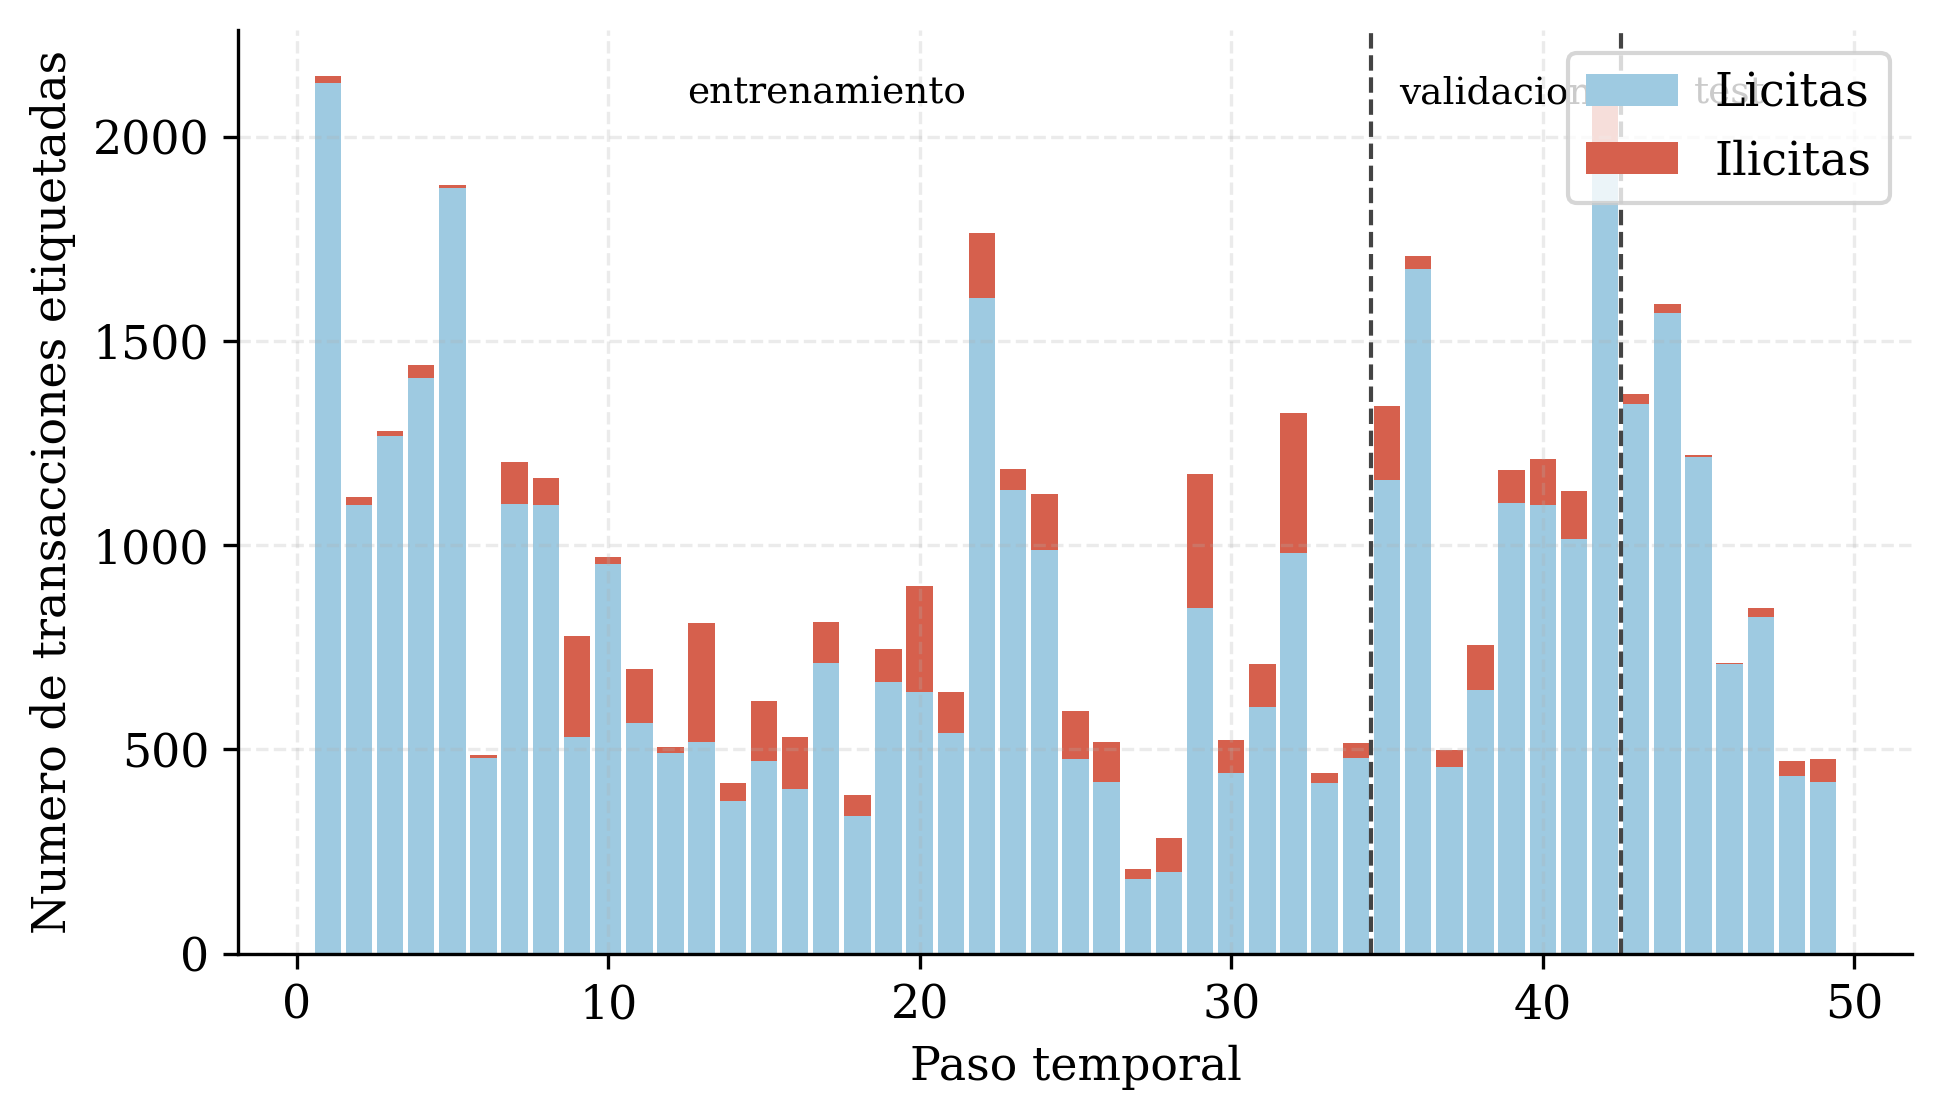
\includegraphics[width=0.85\textwidth]{chapter_4/images_ch4/eda_clases_timestep.png}
    \caption{Distribución de las transacciones etiquetadas del \textit{Elliptic Dataset} a lo largo de los 49 pasos temporales, con las particiones de entrenamiento, validación y test delimitadas. Tanto el volumen total como la proporción de actividad ilícita varían entre periodos, lo que anticipa el desplazamiento temporal que degrada la generalización.}
    \label{fig:eda-clases}
\end{figure}

La estructura temporal del conjunto tiene una implicación que se retoma en la Sección 4.4, la de que los patrones que caracterizan la actividad ilícita no son estacionarios. Un modelo que aprende a discriminar transacciones ilícitas en los primeros pasos temporales se enfrenta, en los últimos pasos, a una distribución que ha cambiado, lo que anticipa la dificultad de generalizar del periodo de entrenamiento al de test. Esta no estacionariedad es una propiedad del fenómeno del lavado, cuyas tipologías evolucionan para evadir la detección, y no un defecto del conjunto de datos. Reconocerla desde el análisis exploratorio permite interpretar correctamente los resultados de rendimiento que se presentan más adelante.

\subsection{Dispersión de la Topología}

Una segunda propiedad del grafo resulta determinante para el resto del estudio y merece un análisis detallado, la dispersión extrema de su topología. La mayoría de los nodos poseen muy pocas conexiones, hasta el punto de que el grado mediano es de dos y el nonagésimo percentil se sitúa en tres, con una media de dos coma tres aristas por nodo, tal como ilustra la Figura \ref{fig:eda-grados}. La escasez es aún más marcada en la clase ilícita, ya que el noventa y tres coma dos por ciento de las transacciones ilícitas presentan dos aristas o menos. Esta característica no es un defecto del preprocesamiento sino una propiedad intrínseca de las transacciones de Bitcoin etiquetadas, y condiciona de manera profunda todo lo que puede medirse sobre las explicaciones.

\begin{figure}[htbp]
    \centering
    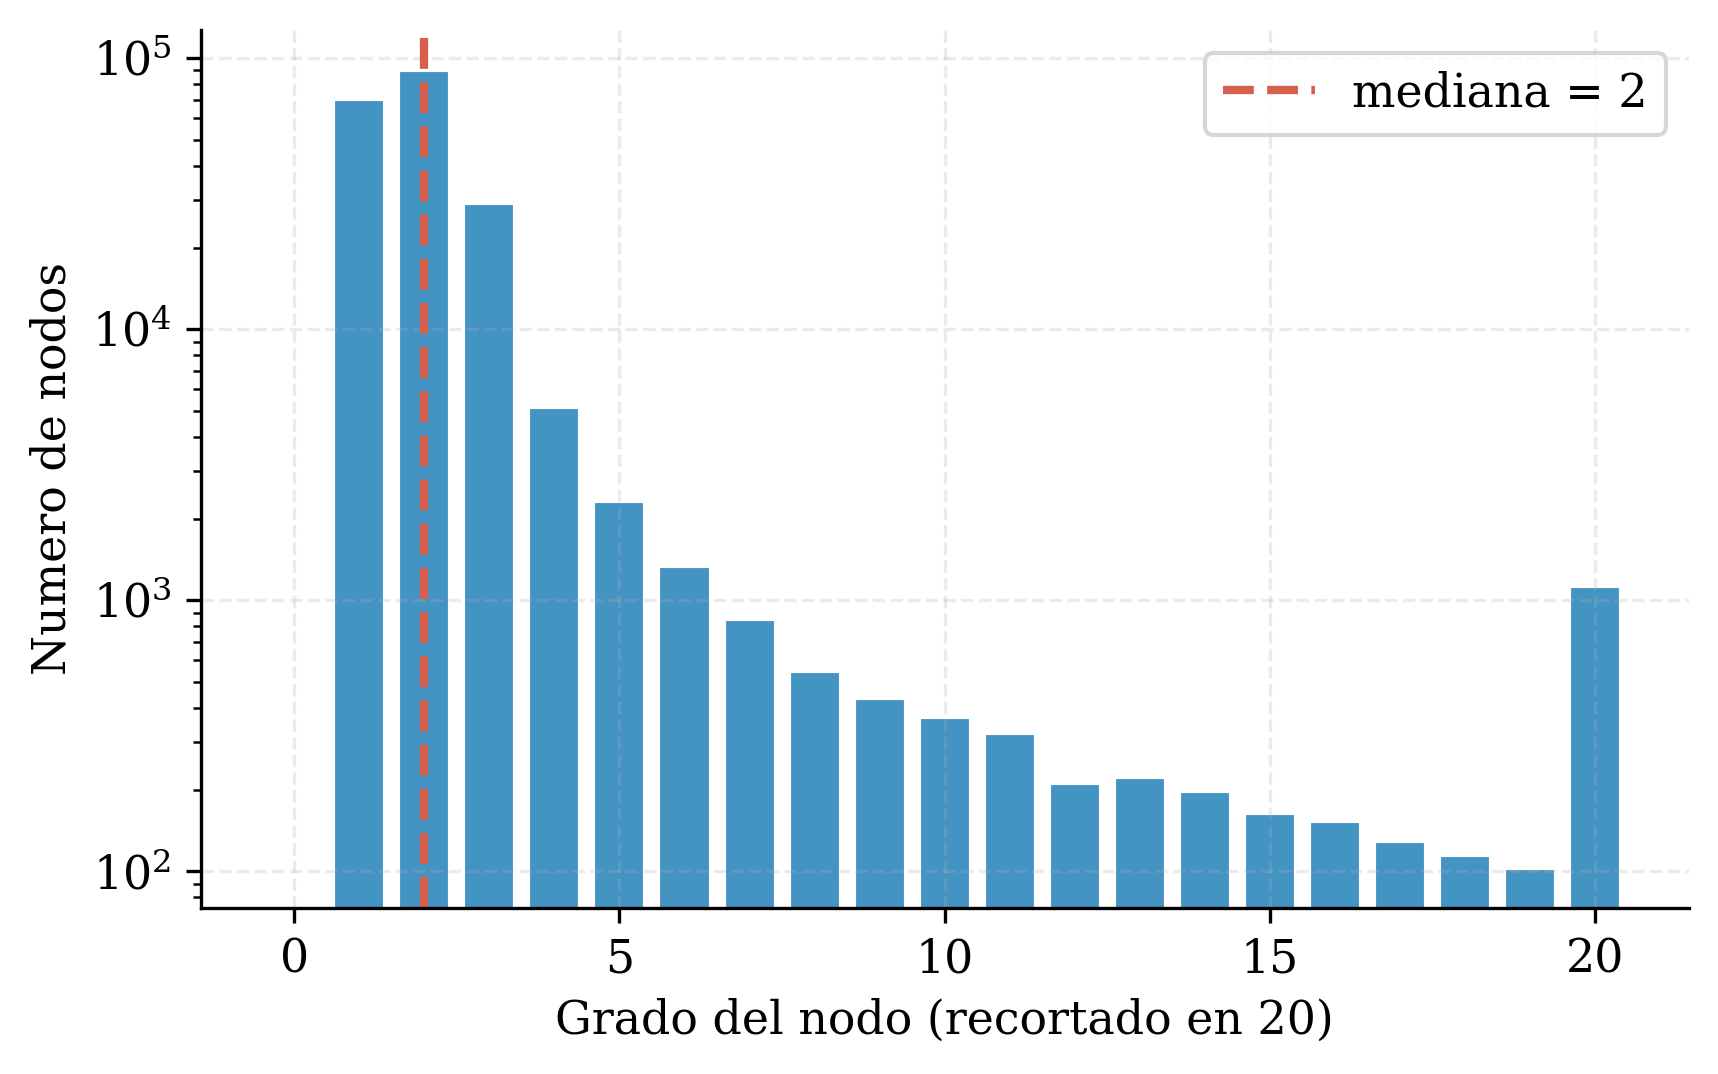
\includegraphics[width=0.75\textwidth]{chapter_4/images_ch4/eda_grados.png}
    \caption{Distribución del grado de los nodos del \textit{Elliptic Dataset} en escala logarítmica, recortada para su visualización. El grado mediano es de dos, lo que evidencia una topología extremadamente dispersa dominada por nodos con muy pocas conexiones.}
    \label{fig:eda-grados}
\end{figure}

La consecuencia directa de esta dispersión se aprecia al construir el subgrafo receptivo de un nodo, es decir el conjunto de nodos que influyen en su predicción a través del paso de mensajes. La mediana del tamaño de ese subgrafo es de apenas dos nodos, como muestra la Figura \ref{fig:dispersion}, de modo que un vecindario tan reducido deja muy poco margen para que una explicación estructural sea informativa o para que su plausibilidad sea medible. Esta limitación es la razón de fondo por la que el eje sintético del Capítulo 5 resulta necesario, ya que sin estructura de subgrafo no existe un patrón que una explicación pueda recuperar ni contra el cual pueda contrastarse.

\begin{figure}[htbp]
    \centering
    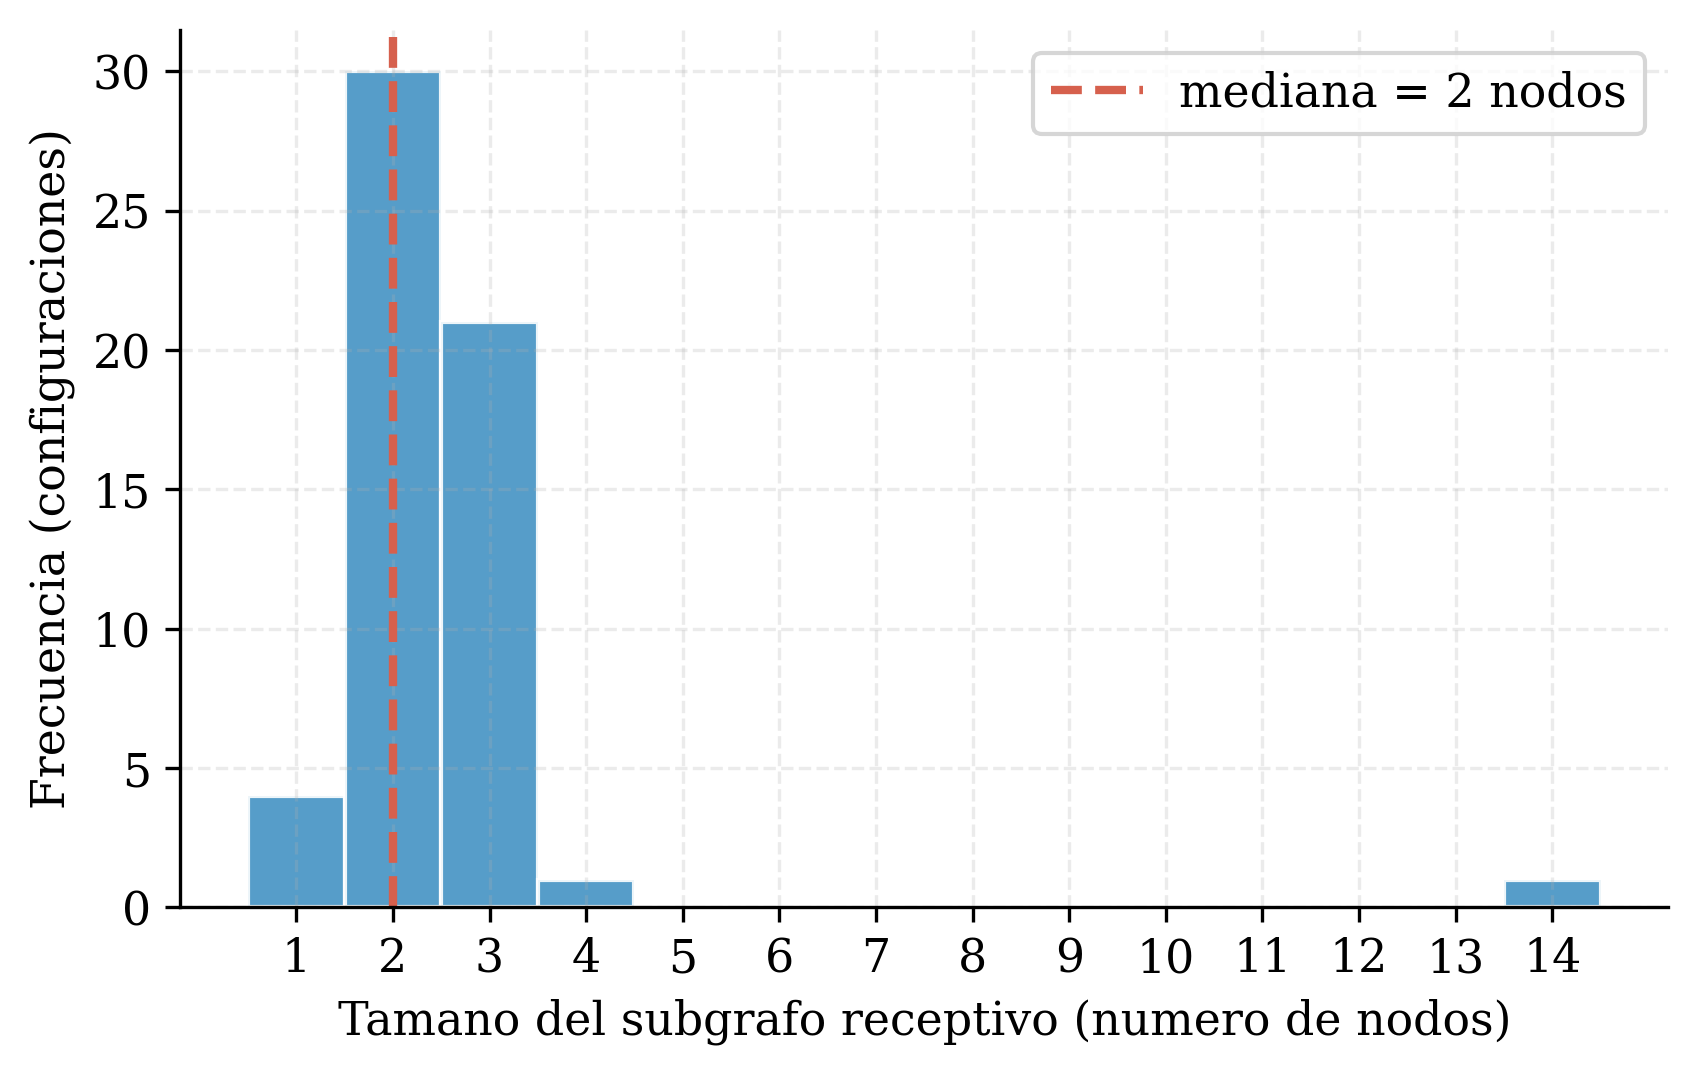
\includegraphics[width=0.8\textwidth]{chapter_4/images_ch4/dispersion_elliptic.png}
    \caption{Distribución del tamaño del subgrafo receptivo de los nodos ilícitos en el \textit{Elliptic Dataset}. La mediana se sitúa en dos nodos, lo que evidencia la dispersión extrema del grafo y explica por qué la plausibilidad estructural de las explicaciones no es medible en este dominio.}
    \label{fig:dispersion}
\end{figure}

La consecuencia inmediata de esta dispersión sobre la evaluación de estabilidad es que el índice de Jaccard entre aristas explicativas pierde buena parte de su capacidad de discriminar. Cuando el subgrafo receptivo contiene una o dos aristas, cualquier método que seleccione las aristas más relevantes recupera el mismo conjunto en cada ejecución, de modo que el índice de Jaccard se satura hacia valores altos, cercano a la unidad en los subgrafos más pequeños, y su media se mantiene comprimida alrededor de valores elevados con independencia de la arquitectura. La Tabla \ref{tab:jaccard} ilustra este efecto, ya que el Jaccard medio apenas varía entre arquitecturas, mientras que la correlación de Spearman de features se distribuye en un rango mucho más amplio y logra distinguir entre ellas. Por esta razón, y como se anticipó en el Capítulo 3, la correlación de Spearman entre los rankings de importancia de las features se adopta como la métrica de estabilidad informativa para el \textit{Elliptic Dataset}, dado que conserva sensibilidad incluso en vecindarios minúsculos, decisión metodológica que condiciona la lectura de todos los resultados de estabilidad que siguen.

\begin{table}[htbp]
\centering
\renewcommand{\arraystretch}{1.3}
\begin{tabular}{lcc}
\toprule
\textbf{Arquitectura} & \textbf{Jaccard medio} & \textbf{Spearman medio} \\
\midrule
GraphSAGE & 0,911 & 0,735 \\
GAT & 0,791 & 0,780 \\
GCN & 0,613 & 0,778 \\
TAGCN & 0,805 & 0,580 \\
\bottomrule
\end{tabular}
\caption{Comparación entre el índice de Jaccard de aristas y la correlación de Spearman de features (GNNExplainer) como métricas de estabilidad sobre el \textit{Elliptic Dataset}, con la métrica corregida. El Jaccard se satura hacia valores altos por la dispersión del grafo, mientras que la correlación de Spearman conserva capacidad de discriminación entre arquitecturas.}
\label{tab:jaccard}
\end{table}


\section{Pipeline Experimental y Espacio Factorial}

El diseño experimental se organiza como una matriz factorial que cruza cuatro dimensiones, a saber las cuatro arquitecturas GNN caracterizadas en el Capítulo 3, un conjunto de escenarios de desbalance, tres estrategias de balanceo y los tres métodos de explicabilidad. Las arquitecturas evaluadas son GCN, GraphSAGE, GAT y TAGCN, y ninguna recibe un tratamiento privilegiado dentro de la comparación. Las estrategias de balanceo comprenden el entrenamiento sin intervención, la ponderación de clases inversamente proporcional a su frecuencia y la Focal Loss \cite{Lin2017FocalDetection}, mientras que los explicadores son GNNExplainer, PGExplainer y GNNShap \cite{Ying2019Gnnexplainer:Networks, Luo2020ParameterizedNetwork, Akkas2024Gnnshap:Values}. El pipeline sigue cuatro fases, la preparación de los datos, el entrenamiento de los modelos con búsqueda de hiperparámetros, la generación de explicaciones y la medición de estabilidad mediante réplicas, tal como resume la Figura \ref{fig:metodologia}.

\begin{figure}[htbp]
    \centering
    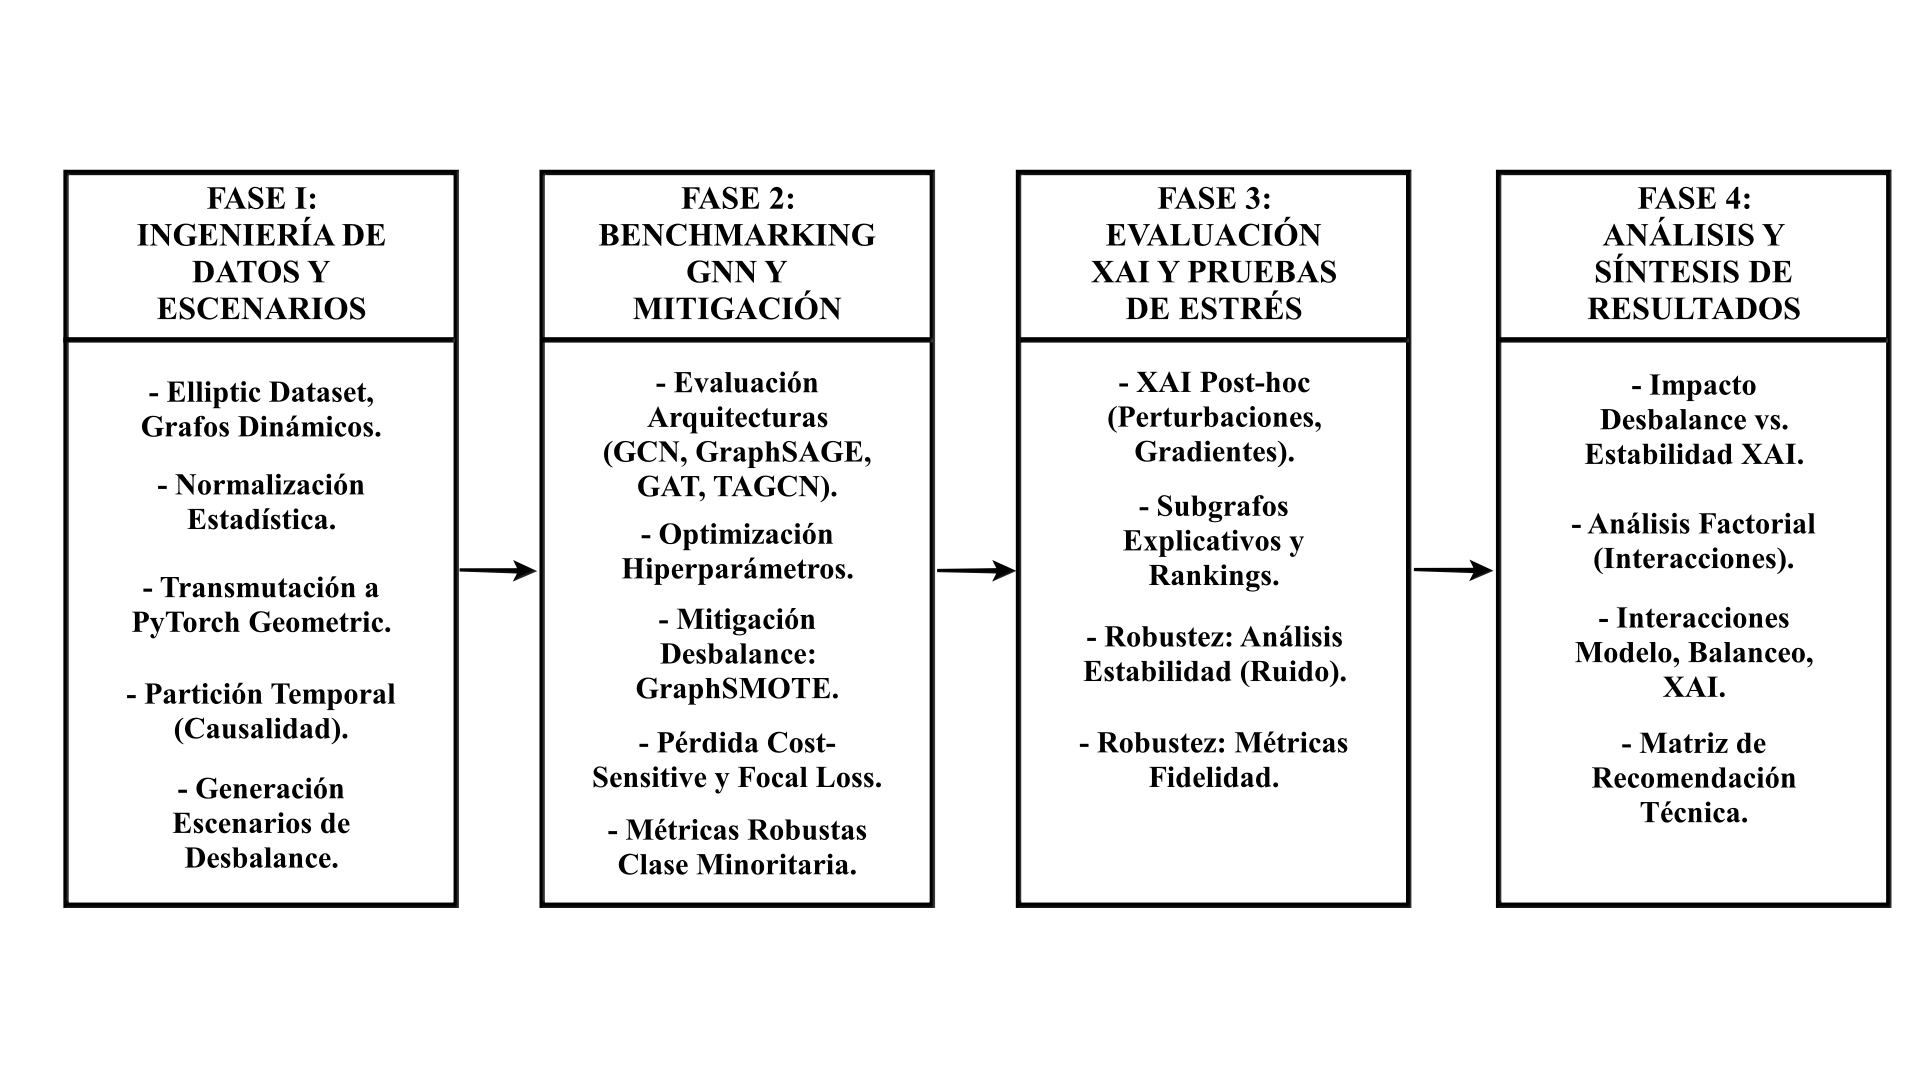
\includegraphics[width=0.9\textwidth]{chapter_4/images_ch4/metodologia.png}
    \caption{Metodología de cuatro fases del pipeline experimental, desde la preparación de los datos hasta la medición de estabilidad de las explicaciones mediante réplicas.}
    \label{fig:metodologia}
\end{figure}

El entrenamiento de cada modelo incorpora una búsqueda de hiperparámetros mediante optimización bayesiana, que ajusta la dimensión de las capas ocultas, el número de capas, la tasa de \textit{dropout} y la tasa de aprendizaje. La métrica que guía la búsqueda es el área bajo la curva de precisión y exhaustividad, más adecuada que la exactitud en presencia de desbalance extremo, y el criterio de parada temprana vigila el F1 de la clase ilícita para evitar detenerse por ruido. Este procedimiento busca que cada configuración alcance la mejor calidad posible antes de generar explicaciones, de manera que la estabilidad se mida sobre modelos que efectivamente aprendieron a discriminar y no sobre clasificadores triviales. La medición de estabilidad repite la explicación de cada nodo de interés cinco veces con semillas distintas y resume la variación resultante mediante la correlación de Spearman de los rankings de features.

\subsection{Compuerta de Calidad y Selección de Nodos a Explicar}

Un principio metodológico atraviesa todo el pipeline, el de que solo tiene sentido estudiar la estabilidad de las explicaciones de modelos que efectivamente aprendieron a discriminar. Para hacerlo operativo, cada configuración debe superar una compuerta de calidad antes de que se generen sus explicaciones, definida sobre la partición de validación mediante dos umbrales, un F1 de la clase ilícita no inferior a treinta centésimas y un coeficiente de correlación de Matthews no inferior a quince centésimas. Las configuraciones que no alcanzan estos umbrales se registran, pero se excluyen del subconjunto sobre el que se afirman las conclusiones, lo que evita que la estabilidad se mida sobre clasificadores triviales cuyas explicaciones carecen de significado. Esta compuerta es la razón por la que el ranking de estabilidad se presenta más adelante en dos corridas, una completa y otra restringida a las configuraciones que superan el filtro.

La selección de los nodos que se explican sigue el mismo principio de significado. Para cada configuración, se explican los nodos de la partición de validación que el modelo clasifica correctamente como ilícitos, es decir los verdaderos positivos, ya que solo en ellos existe una predicción positiva cuya explicación tiene interés analítico. Este criterio garantiza que la estabilidad medida corresponda a explicaciones de aciertos y no de errores, y que la comparación entre arquitecturas y explicadores se realice sobre un conjunto de nodos homogéneo en su condición de verdaderos positivos. El número de verdaderos positivos disponibles varía entre configuraciones, y ese número se registra junto con cada resultado para poder ponderar la confianza de las medias reportadas, tal como se detalla en la tabla completa del anexo.

\section{Escenarios de Desbalance}

Para estudiar el efecto del desbalance de clases sobre la estabilidad, el conjunto de entrenamiento se resamplea en cinco escenarios de proporción creciente entre transacciones ilícitas y lícitas. Los escenarios controlados corresponden a las razones 1:1, 1:10, 1:50 y 1:100, obtenidas mediante submuestreo de la clase mayoritaria, y se añade un escenario nativo que conserva la proporción del subconjunto etiquetado sin aplicar resampleo, cercana a 1:9. Esta gradación permite observar si la estabilidad de las explicaciones se degrada de forma monótona a medida que la clase ilícita se vuelve más escasa, o si presenta un comportamiento distinto. La inclusión del escenario nativo resulta relevante porque representa la condición realista del dato, sin manipulación artificial de la proporción, y ofrece un punto de comparación frente a los escenarios construidos.

\section{Rendimiento Predictivo y el Colapso de Validación a Test}

La evaluación del rendimiento bajo un desbalance tan extremo exige elegir la métrica con cuidado, puesto que el F1 calculado sobre un umbral fijo se vuelve degenerado cuando la clase positiva representa una fracción mínima del total. Por esa razón, la métrica primaria de este estudio es el área bajo la curva de precisión y exhaustividad, que resume la capacidad de ordenamiento del modelo sin depender de un umbral y que coincide con la magnitud pertinente en la práctica de la auditoría antilavado, donde el analista revisa un conjunto acotado de alertas de mayor puntuación en lugar de una decisión binaria sobre todo el universo de transacciones. Bajo esta métrica, los modelos alcanzan un rendimiento razonable sobre la partición de validación, con un valor de 0,52 en la mejor configuración hallada por la búsqueda de hiperparámetros y una media de 0,367 sobre los modelos que superan el filtro de calidad, lo que indica que el modelo aprende a situar las transacciones ilícitas por encima de las lícitas en el ordenamiento. Ese desempeño no se traslada a la partición de test, donde el área bajo la misma curva cae a un valor medio cercano a 0,013 sobre el conjunto de las sesenta configuraciones, y de 0,017 sobre las que superan el filtro de calidad, una caída que ninguna arquitectura evita y que el F1 en test, prácticamente nulo en las cuatro arquitecturas con valores de 0,0245 para GAT, 0,0133 para GCN, 0,0077 para GraphSAGE y 0,0015 para TAGCN, no hace sino reflejar de forma todavía más marcada, tal como recoge la Tabla \ref{tab:elliptic-perf}. Este fenómeno, que puede denominarse colapso de validación a test, constituye uno de los rasgos más importantes del dominio y condiciona la interpretación de todo el estudio.

\begin{table}[htbp]
\centering
\renewcommand{\arraystretch}{1.3}
\begin{tabular}{lccc}
\toprule
\textbf{Arquitectura} & \textbf{F1 (test)} & \textbf{MCC (test)} & \textbf{PR-AUC (test)} \\
\midrule
GraphSAGE & 0,008 & 0,003 & 0,017 \\
GAT & 0,025 & 0,017 & 0,014 \\
GCN & 0,013 & 0,008 & 0,010 \\
TAGCN & 0,001 & -0,006 & 0,011 \\
\bottomrule
\end{tabular}
\caption{Rendimiento predictivo medio en la particion de test por arquitectura sobre el \textit{Elliptic Dataset}. El colapso es generalizado, con valores de F1 y MCC muy bajos en las cuatro arquitecturas por efecto del desplazamiento temporal.}
\label{tab:elliptic-perf}
\end{table}


Para dimensionar el colapso con una perspectiva complementaria, se recalcularon sobre las particiones de validación y test dos familias de métricas de ordenamiento, el área bajo la curva ROC y la precisión en los primeros nodos de mayor puntuación, junto al área bajo la curva de precisión y exhaustividad, cuyos valores medios recoge la Tabla \ref{tab:elliptic-rocauc}. El contraste entre ellas es en sí mismo instructivo y refuerza la elección de la métrica primaria. Sobre validación, los modelos que superan el filtro de calidad alcanzan un ROC-AUC medio de 0,884 que sugeriría un clasificador casi excelente, pero el mismo conjunto arroja un área de precisión y exhaustividad de 0,367 y una precisión en los primeros cincuenta nodos de 0,657, cifras que revelan una tarea mucho más difícil de lo que el ROC-AUC insinúa. Sobre test la disociación se vuelve extrema, ya que el ROC-AUC se mantiene en 0,653, un valor que por sí solo parecería indicar un modelo apenas mediocre, mientras que el área de precisión y exhaustividad se desploma a 0,017 y la precisión en los primeros cincuenta nodos a 0,020, apenas por encima de la tasa base de transacciones ilícitas en el test. Esta discrepancia ilustra por qué el ROC-AUC resulta engañoso bajo desbalance extremo, puesto que su eje de tasa de falsos positivos queda dominado por la enorme clase mayoritaria y permanece bajo aunque el modelo no distinga la clase rara, lo que justifica adoptar el área de precisión y exhaustividad y la precisión en los primeros nodos como métricas primarias, que son ademas las que gobiernan el trabajo real de triaje en una auditoría antilavado.

\begin{table}[htbp]
\centering
\renewcommand{\arraystretch}{1.3}
\begin{tabular}{lcc}
\toprule
\textbf{Métrica de ordenamiento} & \textbf{Validación} & \textbf{Test} \\
\midrule
ROC-AUC & 0,884 & 0,653 \\
PR-AUC & 0,367 & 0,017 \\
Precisión en los primeros 50 & 0,657 & 0,020 \\
Precisión en los primeros 100 & 0,640 & 0,022 \\
\bottomrule
\end{tabular}
\caption{Métricas de ordenamiento medias sobre validación y test para los modelos que superan el filtro de calidad. El ROC-AUC se mantiene alto y engañoso bajo el desbalance extremo, mientras que el área de precisión y exhaustividad y la precisión en los primeros nodos revelan la dificultad real de la tarea y el colapso en test.}
\label{tab:elliptic-rocauc}
\end{table}

La causa del colapso no reside en un defecto del método sino en una propiedad estructural del dato, el desplazamiento temporal entre las particiones. El \textit{Elliptic Dataset} ordena las transacciones por pasos temporales, y los patrones que caracterizan la actividad ilícita en los primeros pasos difieren de los que aparecen en los últimos, de modo que un modelo ajustado sobre el periodo de validación encuentra en test una distribución distinta a la que aprendió \cite{Menezes2025SemanticDetectors}. Trabajos previos sobre el mismo conjunto de datos han documentado la fragilidad de los detectores basados en grafos ante este tipo de desplazamiento, lo que refuerza que se trata de una limitación del dato y no de la implementación \cite{Lawal2025AnDataset}. Reconocer esta limitación de forma explícita es preferible a ocultarla, ya que delimita con honestidad el alcance de las conclusiones. En consecuencia, y puesto que el objeto de la tesis es la estabilidad de las explicaciones y no el rendimiento predictivo en test, el estudio de estabilidad se realiza sobre los nodos de la partición de validación que el modelo clasifica correctamente como ilícitos.

Conviene precisar el sentido de esta decisión para evitar malentendidos. Estudiar la estabilidad sobre validación no busca disimular el colapso, sino situar el análisis allí donde el modelo efectivamente discrimina y donde, por tanto, la pregunta por la estabilidad de una explicación tiene sentido. Un modelo que no detecta ninguna transacción ilícita en test no genera predicciones positivas cuya explicación pueda evaluarse, de manera que forzar la medición sobre test produciría explicaciones de predicciones erróneas y carentes de interés analítico. La estabilidad reportada en las secciones siguientes se refiere, por tanto, a las explicaciones de verdaderos positivos sobre validación, un encuadre que se declara de forma transparente y que constituye una respuesta metodológica honesta ante una limitación estructural del dato.

\section{De un Artefacto de Cómputo a un Artefacto de Medida: dos Correcciones Metodológicas}

La forma en que se generan las explicaciones tiene un efecto inesperado y de gran alcance sobre los resultados de estabilidad. En una primera versión del pipeline, cada explicación se calculaba sobre el grafo completo de 203.769 nodos, lo que imponía una carga de memoria considerable a los explicadores basados en máscaras. En el caso de GAT, cuyo mecanismo de atención multiplica el consumo de memoria por el número de cabezas, esa carga provocaba fallos por agotamiento de memoria de la unidad de procesamiento gráfico, con picos cercanos a 7,5 GiB. El problema más serio no era el fallo en sí, sino que trece de esas configuraciones de GAT fallaban de forma silenciosa y sus filas quedaban vacías, de modo que el promedio de estabilidad de GAT terminaba calculándose solo sobre las siete u ocho configuraciones que sí completaban la ejecución.

Este comportamiento generaba un artefacto grave que conviene exponer con detalle. El ranking de estabilidad de la versión anterior situaba a GAT como la arquitectura más estable, con un valor cercano a 0,534, por encima de GraphSAGE, que aparecía como la peor con 0,345, pero esa comparación no era legítima porque GAT se medía sobre un subconjunto favorable de sus configuraciones mientras GraphSAGE se medía sobre todas. La primera corrección consiste en calcular cada explicación sobre el subgrafo receptivo del nodo de interés, es decir el conjunto de nodos que realmente influyen en su predicción según el número de capas de la arquitectura, en lugar de sobre el grafo completo. Para TAGCN, cuyo campo receptivo se amplía por el orden del filtro polinomial, se emplea un radio de dos saltos. Esta restricción reduce el consumo de memoria de 7,5 GiB a 0,02 GiB y elimina por completo los fallos, de manera que las cuatro arquitecturas pasan a medirse sobre el mismo soporte y en condiciones equitativas.

La medición sobre el subgrafo receptivo, con todo, seguía descansando sobre una implementación defectuosa de la propia métrica de estabilidad, cuya reparación constituye la segunda corrección. La correlación de Spearman entre rankings de features se calculaba descartando toda feature cuyo índice superara el parámetro de truncamiento, fijado en veinte para el Elliptic Dataset, lo que equivalía a comparar rankings mutilados y deprimía de forma sistemática la concordancia medida. La reparación conserva la longitud completa de cada ranking y asigna un rango común a las features situadas fuera del conjunto principal, en lugar de eliminarlas. Un rasgo decisivo para la interpretación es que el efecto de esta reparación no es uniforme entre arquitecturas, porque el truncamiento penalizaba con mayor severidad a aquellas cuya importancia se reparte sobre un número mayor de features.

Al recomputar la estabilidad con la métrica corregida sobre el subconjunto de veintitrés configuraciones que superan el filtro de calidad, el mismo que la tesis utiliza para sus conclusiones, la ventaja de GraphSAGE desaparece y el orden vuelve a modificarse. GAT alcanza una correlación media de 0,779 sobre siete configuraciones, por encima de GraphSAGE con 0,743 sobre once, mientras que GCN queda en 0,833 sobre una única configuración y TAGCN en 0,641 sobre cuatro, tal como recoge la Tabla \ref{tab:ranking} y visualiza la Figura \ref{fig:ranking}. La reparación elevó a GAT en 0,244 puntos y a TAGCN en 0,278, frente a un ascenso de apenas 0,103 en GraphSAGE, lo que identifica al truncamiento de la métrica como la causa de la aparente superioridad de GraphSAGE que reportaba la versión anterior. La comparación restringida a las siete configuraciones en que GAT y GraphSAGE superan ambos el filtro, un contraste libre de sesgo de selección, sostiene el mismo sentido, puesto que GAT promedia 0,779 frente a 0,739 de GraphSAGE, cuando con la métrica defectuosa el orden era el inverso, de 0,535 frente a 0,627. El mismo orden se observa sobre la corrida completa de las sesenta configuraciones, donde GAT y GCN encabezan con 0,780 y 0,778, por delante de GraphSAGE con 0,735 y de TAGCN con 0,580, lo que confirma que la conclusión no depende del filtro de calidad.

\begin{figure}[htbp]
    \centering
    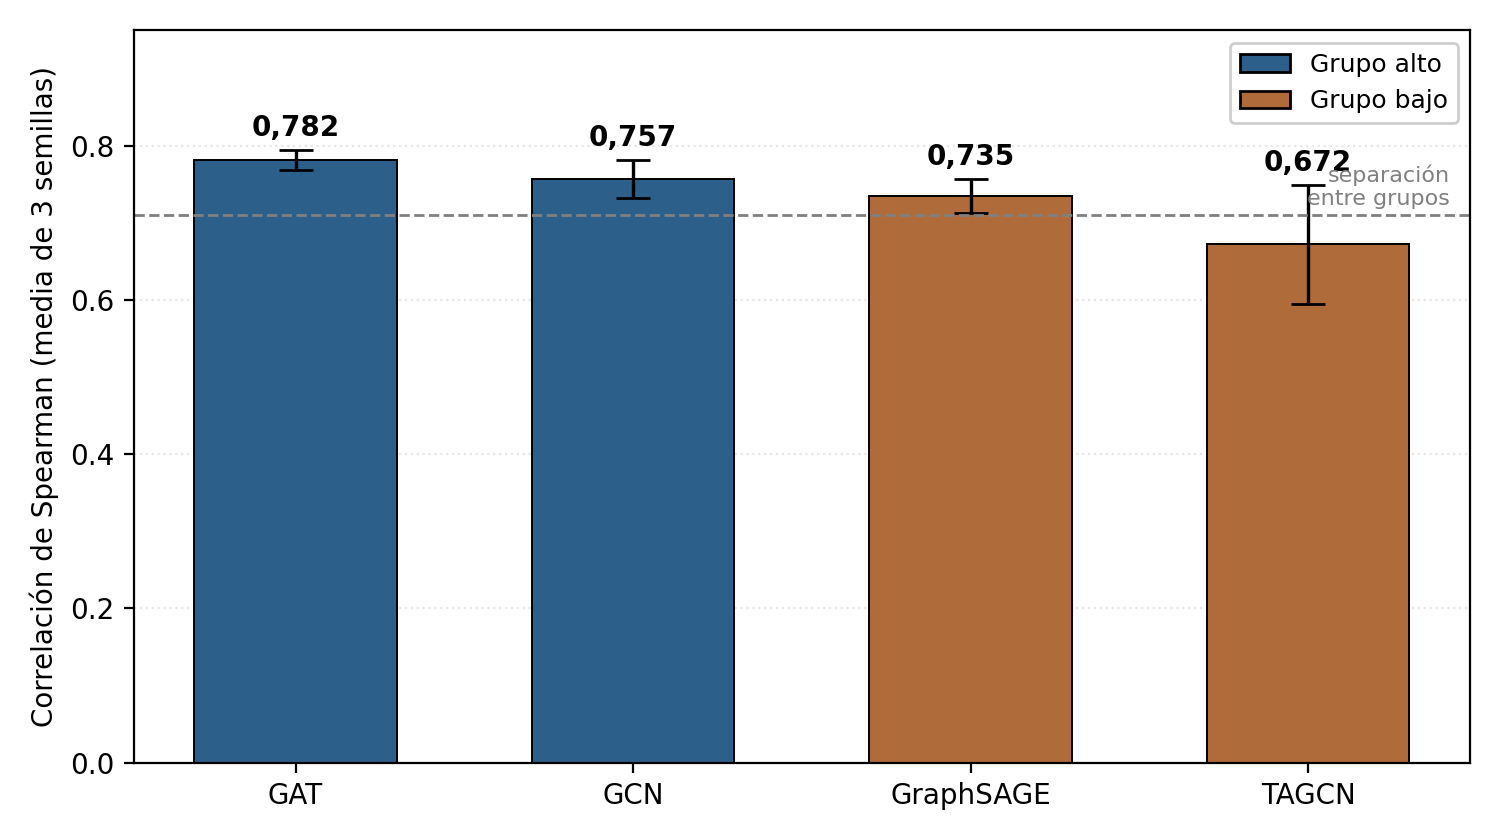
\includegraphics[width=0.85\textwidth]{chapter_4/images_ch4/ranking_khop.png}
    \caption{Estabilidad de las explicaciones por arquitectura sobre el subgrafo receptivo y con la métrica de Spearman corregida, promediada sobre las tres semillas de modelo, con barras de error que representan la desviación típica entre semillas. La prueba de rangos con signo separa un grupo alto formado por GAT y GCN de un grupo bajo formado por GraphSAGE y TAGCN, con diferencias significativas entre grupos y no dentro del grupo bajo. La mayor dispersión de TAGCN advierte contra fijar su valor central con demasiada precisión.}
    \label{fig:ranking}
\end{figure}

La lectura que esta tesis afirma como robusta debe revisarse a la luz de la métrica corregida, y el resultado es más prudente que el de la versión anterior. Ninguna arquitectura domina la estabilidad de forma transversal, y la superioridad de GraphSAGE sobre GAT que la versión previa reportaba no sobrevive a la reparación de la métrica. Sobre el subconjunto con calidad garantizada, GAT y GraphSAGE resultan prácticamente indistinguibles, con una diferencia de cuatro centésimas sostenida sobre siete y once configuraciones, mientras que GCN se apoya en una sola configuración y TAGCN en cuatro, un soporte insuficiente para fijar su posición relativa. La afirmación que sí se sostiene, y que gana fuerza al contrastarse con el eje sintético del Capítulo 5, es que el orden de estabilidad corregido en Elliptic concuerda con el del grafo denso, en el que GCN y GAT encabezan la estabilidad de GNNExplainer, de modo que la resiliencia de estas arquitecturas se manifiesta con relativa independencia de la densidad del grafo.

La prudencia de esta lectura se apoya en un contraste estadístico explícito. La diferencia de estabilidad entre GAT y GraphSAGE sobre las siete configuraciones en que ambos superan el filtro, de apenas cuatro centésimas, no alcanza significación estadística, ni con la prueba de rangos con signo de Wilcoxon, que arroja un valor p de 0,375, ni con la prueba t pareada, con un valor p de 0,380. Los intervalos de confianza al noventa y cinco por ciento de sus medias se solapan de forma amplia, de 0,705 a 0,853 para GAT y de 0,720 a 0,766 para GraphSAGE. Conviene subrayar el origen de esta indeterminación, que no reside en que las arquitecturas sean equivalentes sino en que una sola inicialización sobre un soporte reducido carece de potencia para separarlas. La sección siguiente levanta precisamente esa limitación mediante una replicación con tres semillas de modelo, y con ella la comparación entre GAT y GraphSAGE sí alcanza significación, de manera que la cautela expresada aquí debe leerse como una restricción del diseño de una sola semilla y no como una conclusión sobre las arquitecturas.

La sucesión de las dos correcciones encierra un valor metodológico que trasciende el resultado puntual. Un primer artefacto, de naturaleza computacional, favorecía a GAT mediante un cálculo sobre el grafo completo que fallaba de forma silenciosa y dejaba fuera sus configuraciones más costosas; un segundo artefacto, de naturaleza métrica, favorecía a GraphSAGE mediante un truncamiento que mutilaba los rankings de features y penalizaba con más fuerza a las arquitecturas de importancia más repartida. Cada uno de ellos, por separado, bastaba para producir una conclusión comparativa llamativa y falsa, y solo la corrección de ambos permite una lectura estable de los datos. Este doble episodio ilustra de forma concreta la advertencia de Kosan y colaboradores sobre la sensibilidad de las conclusiones al protocolo de evaluación, y refuerza la necesidad de auditar las condiciones de cómputo y de medida con el mismo rigor que se aplica a los métodos \cite{Kosan2023GNNX-BENCH:Benchmarking}.

\section{Replicación con Múltiples Semillas y Estructura en Dos Grupos}

Las conclusiones expuestas hasta aquí descansaban sobre una única inicialización del entrenamiento, lo que impedía separar una diferencia real entre arquitecturas del ruido propio de un ajuste concreto. Para levantar esa limitación, la matriz completa de sesenta configuraciones se reentrenó con tres semillas de modelo independientes, cada una ejecutando el procedimiento entero, incluida su propia búsqueda de hiperparámetros, hasta totalizar ciento ochenta modelos sobre los que se recalculó la estabilidad de GNNExplainer. Mantener la búsqueda dentro de la replicación, en lugar de reutilizar los hiperparámetros de la primera semilla, responde al propósito de medir la variabilidad del procedimiento completo y no solo la de la inicialización de los pesos, que es la pregunta pertinente cuando lo que se desea establecer es si una conclusión depende de una corrida particular.

La replicación arroja en primer término un resultado sobre reproducibilidad que conviene declarar con precisión. Reentrenar con la misma semilla no devuelve modelos idénticos, ya que las operaciones de dispersión que implementan el paso de mensajes sobre la unidad de procesamiento gráfico emplean sumas atómicas cuyo orden no es determinista, de modo que la reproducibilidad exacta a nivel de pesos no es alcanzable sin renunciar al rendimiento. Lo que sí se reproduce, y es lo que importa para una afirmación científica, son las conclusiones, puesto que el reentrenamiento independiente de la matriz devolvió el mismo filtro de calidad, con veinticinco configuraciones superándolo frente a las veintitrés originales, y el mismo orden de estabilidad entre arquitecturas. La distinción entre reproducibilidad de los pesos y reproducibilidad de las conclusiones es pertinente para cualquier trabajo que entrene redes sobre grafos en aceleradores gráficos, y omitirla induce expectativas que el cómputo no puede satisfacer.

Los valores medios por arquitectura y semilla, que recoge la Tabla \ref{tab:seeds}, sostienen el orden reportado en la sección anterior y a la vez precisan su lectura. GAT encabeza con una media de 0,782 y una desviación típica de 0,013, seguido de GCN con 0,757, GraphSAGE con 0,735 y TAGCN con 0,672. Las dos primeras posiciones se permutan entre semillas, ya que GCN encabeza en una de ellas y GAT en las otras dos, lo que confirma de forma empírica la cautela con la que la sección anterior se negaba a nombrar una única arquitectura ganadora. TAGCN, por su parte, resulta ser la arquitectura con mayor dispersión entre semillas con diferencia, con una desviación típica de 0,077 frente a valores comprendidos entre 0,013 y 0,025 en las restantes, de manera que el valor de 0,580 que arrojaba la semilla única correspondía al extremo bajo de su rango y no a su comportamiento típico.

\begin{table}[htbp]
    \centering
    \renewcommand{\arraystretch}{1.3}
    \begin{tabular}{lccccc}
    \toprule
    \textbf{Arquitectura} & \textbf{Semilla 42} & \textbf{Semilla 43} & \textbf{Semilla 44} & \textbf{Media} & \textbf{Desv. típica} \\
    \midrule
    GAT       & 0,766 & 0,789 & 0,790 & 0,782 & 0,013 \\
    GCN       & 0,783 & 0,733 & 0,757 & 0,757 & 0,025 \\
    GraphSAGE & 0,756 & 0,713 & 0,738 & 0,735 & 0,022 \\
    TAGCN     & 0,586 & 0,693 & 0,736 & 0,672 & 0,077 \\
    \bottomrule
    \end{tabular}
    \caption{Estabilidad media de las explicaciones de GNNExplainer por arquitectura y semilla de modelo sobre el Elliptic Dataset, con la métrica de Spearman corregida. Las dos primeras posiciones se permutan entre semillas, mientras que TAGCN exhibe una dispersión tres veces mayor que la de cualquier otra arquitectura.}
    \label{tab:seeds}
\end{table}

La potencia inferencial que aporta la replicación permite sustituir un ordenamiento de cuatro posiciones por una estructura más simple y mejor sostenida. Sobre las celdas comunes de escenario, balanceo y semilla, la prueba de rangos con signo de Wilcoxon separa con claridad dos grupos. GAT y GCN resultan indistinguibles entre sí, con un valor p de 0,165, y ambos superan de forma significativa a GraphSAGE, con valores p de 0,0033 y 0,047 respectivamente, y a TAGCN, con valores p inferiores a 0,0001 y de 0,0067. En el extremo opuesto, GraphSAGE y TAGCN tampoco se distinguen entre sí, con un valor p de 0,096. La lectura correcta de la estabilidad por arquitectura en Elliptic no es, por tanto, un ranking de cuatro puestos sino una partición en un grupo alto formado por GAT y GCN y un grupo bajo formado por GraphSAGE y TAGCN, con diferencias significativas entre grupos y no dentro de ellos.

La partición resiste además el contraste con una familia de pruebas distinta de la empleada hasta aquí, lo que descarta que sea un artefacto del diseño pareado. La prueba de Kruskal-Wallis sobre las cuatro arquitecturas rechaza la hipótesis de igualdad con un estadístico de 23,79 y un valor p de 2,8 por diez elevado a menos cinco, con un tamaño de efecto epsilon cuadrado de 0,125 que corresponde a una magnitud media. Al aplicar la misma prueba dentro de cada grupo, en cambio, la igualdad no se rechaza, ni entre GAT y GCN, con un valor p de 0,192, ni entre GraphSAGE y TAGCN, con un valor p de 0,080. La comparación no pareada entre el conjunto de las dos arquitecturas del grupo alto y el de las dos del grupo bajo, mediante la prueba de Mann-Whitney, arroja un valor p de 1,4 por diez elevado a menos seis. El patrón es por tanto consistente, ya que la variabilidad entre arquitecturas se concentra entre grupos y no dentro de ellos.

Los intervalos de confianza bootstrap que recoge la Tabla \ref{tab:ic} ofrecen la misma lectura en forma de estimación por intervalo. El intervalo de GAT, de 0,758 a 0,805, y el de GCN, de 0,724 a 0,787, se solapan de forma amplia, al igual que el de GraphSAGE, de 0,710 a 0,756, con el de TAGCN, de 0,632 a 0,717. Entre grupos, en cambio, los intervalos de GAT y de GraphSAGE apenas se tocan, y el de TAGCN es el más ancho de los cuatro, con una amplitud de 0,085 que casi duplica la de GAT y que refleja la mayor dispersión entre semillas ya señalada.

\begin{table}[htbp]
    \centering
    \renewcommand{\arraystretch}{1.3}
    \begin{tabular}{lcccc}
    \toprule
    \textbf{Arquitectura} & \textbf{n} & \textbf{Media} & \textbf{IC95 inferior} & \textbf{IC95 superior} \\
    \midrule
    GAT       & 45 & 0,782 & 0,758 & 0,805 \\
    GCN       & 44 & 0,758 & 0,724 & 0,787 \\
    GraphSAGE & 42 & 0,735 & 0,710 & 0,756 \\
    TAGCN     & 40 & 0,676 & 0,632 & 0,717 \\
    \bottomrule
    \end{tabular}
    \caption{Estabilidad media por arquitectura sobre el Elliptic Dataset e intervalos de confianza al noventa y cinco por ciento obtenidos por remuestreo bootstrap con diez mil réplicas, agregando las tres semillas de modelo. Los intervalos se solapan dentro de cada grupo y apenas se tocan entre grupos, en coherencia con las pruebas de hipótesis. La mayor amplitud del intervalo de TAGCN refleja su elevada dispersión entre semillas.}
    \label{tab:ic}
\end{table}

Esta estructura corrige y a la vez fortalece lo afirmado con una sola semilla. Fortalece, porque la comparación entre GAT y GraphSAGE, que con una semilla no alcanzaba significación y obligaba a una formulación cautelosa, pasa a ser significativa con un valor p de 0,0033, de modo que ahora puede sostenerse que el grupo alto supera al resto y no solamente que lo encabeza. Corrige, porque la afirmación de que TAGCN quedaba netamente rezagada no sobrevive a la replicación, dado que su distancia respecto de GraphSAGE no alcanza significación estadística. Lo que sí se mantiene, y es lo que la hipótesis de trabajo comprometía, es que TAGCN no resulta la arquitectura más estable pese a su alcance multisalto, ya que aparece de forma consistente en el grupo bajo en las tres semillas.

Un último aspecto refuerza la solidez de esta partición. El eje sintético del Capítulo 5, medido de forma independiente sobre un régimen de densidad opuesto y con su propia replicación, exhibe exactamente la misma estructura, con GCN en 0,965 y GAT en 0,960 muy por encima de GraphSAGE en 0,889 y TAGCN en 0,886, valores que separan dos grupos con la misma composición y con diferencias internas mínimas. Que dos regímenes tan distintos, medidos con datos y con pipelines separados, converjan en la misma partición constituye un respaldo considerablemente más fuerte que la coincidencia de un orden entre cuatro posiciones, y refuerza la lectura conjunta que desarrolla el Capítulo 6.

\begin{table}[htbp]
    \centering
    \renewcommand{\arraystretch}{1.3}
    \begin{tabular}{lccc}
    \toprule
    \textbf{Arquitectura} & \textbf{Corrida completa (n)} & \textbf{Corrida con filtro (n)} & \textbf{Tres semillas} \\
    \midrule
    GAT       & 0,780 (15) & 0,779 (7)  & 0,782 $\pm$ 0,013 \\
    GCN       & 0,778 (15) & 0,833 (1)  & 0,757 $\pm$ 0,025 \\
    GraphSAGE & 0,735 (15) & 0,743 (11) & 0,735 $\pm$ 0,022 \\
    TAGCN     & 0,580 (12) & 0,641 (4)  & 0,672 $\pm$ 0,077 \\
    \bottomrule
    \end{tabular}
    \caption{Estabilidad de las explicaciones (correlación de Spearman) por arquitectura sobre el subgrafo receptivo y con la métrica corregida. Las dos primeras columnas corresponden a la semilla original, con el número de configuraciones de soporte entre paréntesis, y la tercera a la media y la desviación típica sobre las tres semillas de la replicación descrita en la sección siguiente. Con la métrica reparada, GAT y GCN encabezan las tres columnas y la anterior ventaja de GraphSAGE no se sostiene. El soporte de la corrida con filtro es desigual, ya que GCN se apoya en una única configuración y TAGCN en cuatro, de modo que esa columna se reporta como control de consistencia y no como estimación. La replicación resuelve esa limitación y sitúa a TAGCN en 0,672, bastante por encima del valor que arrojaba la semilla única, además de revelar que es la arquitectura con mayor dispersión entre semillas.}
    \label{tab:ranking}
\end{table}

El comportamiento de la estabilidad a lo largo de los escenarios de desbalance confirma que este factor no gobierna la reproducibilidad de las explicaciones. Con la métrica corregida, el perfil es esencialmente plano, con valores medios que van de 0,709 en el escenario nativo a 0,741 en el escenario 1:100, pasando por 0,723 en 1:1, 0,726 en 1:10 y 0,727 en 1:50, como ilustra la Figura \ref{fig:escenario} y detalla por arquitectura la Tabla \ref{tab:elliptic-stab-scen}. La amplitud total entre escenarios, de apenas tres centésimas, indica que el nivel de desbalance no produce un deterioro monótono ni un punto de quiebre localizado. En consecuencia desaparece tanto el supuesto pico de inestabilidad en el escenario 1:50 como cualquier paradoja atribuida al escenario nativo, ya que ningún punto destaca sobre los demás. Esta planitud resulta coherente con el hallazgo, desarrollado en el eje sintético, de que el desbalance es un factor secundario frente al explicador y la arquitectura.

\begin{figure}[htbp]
    \centering
    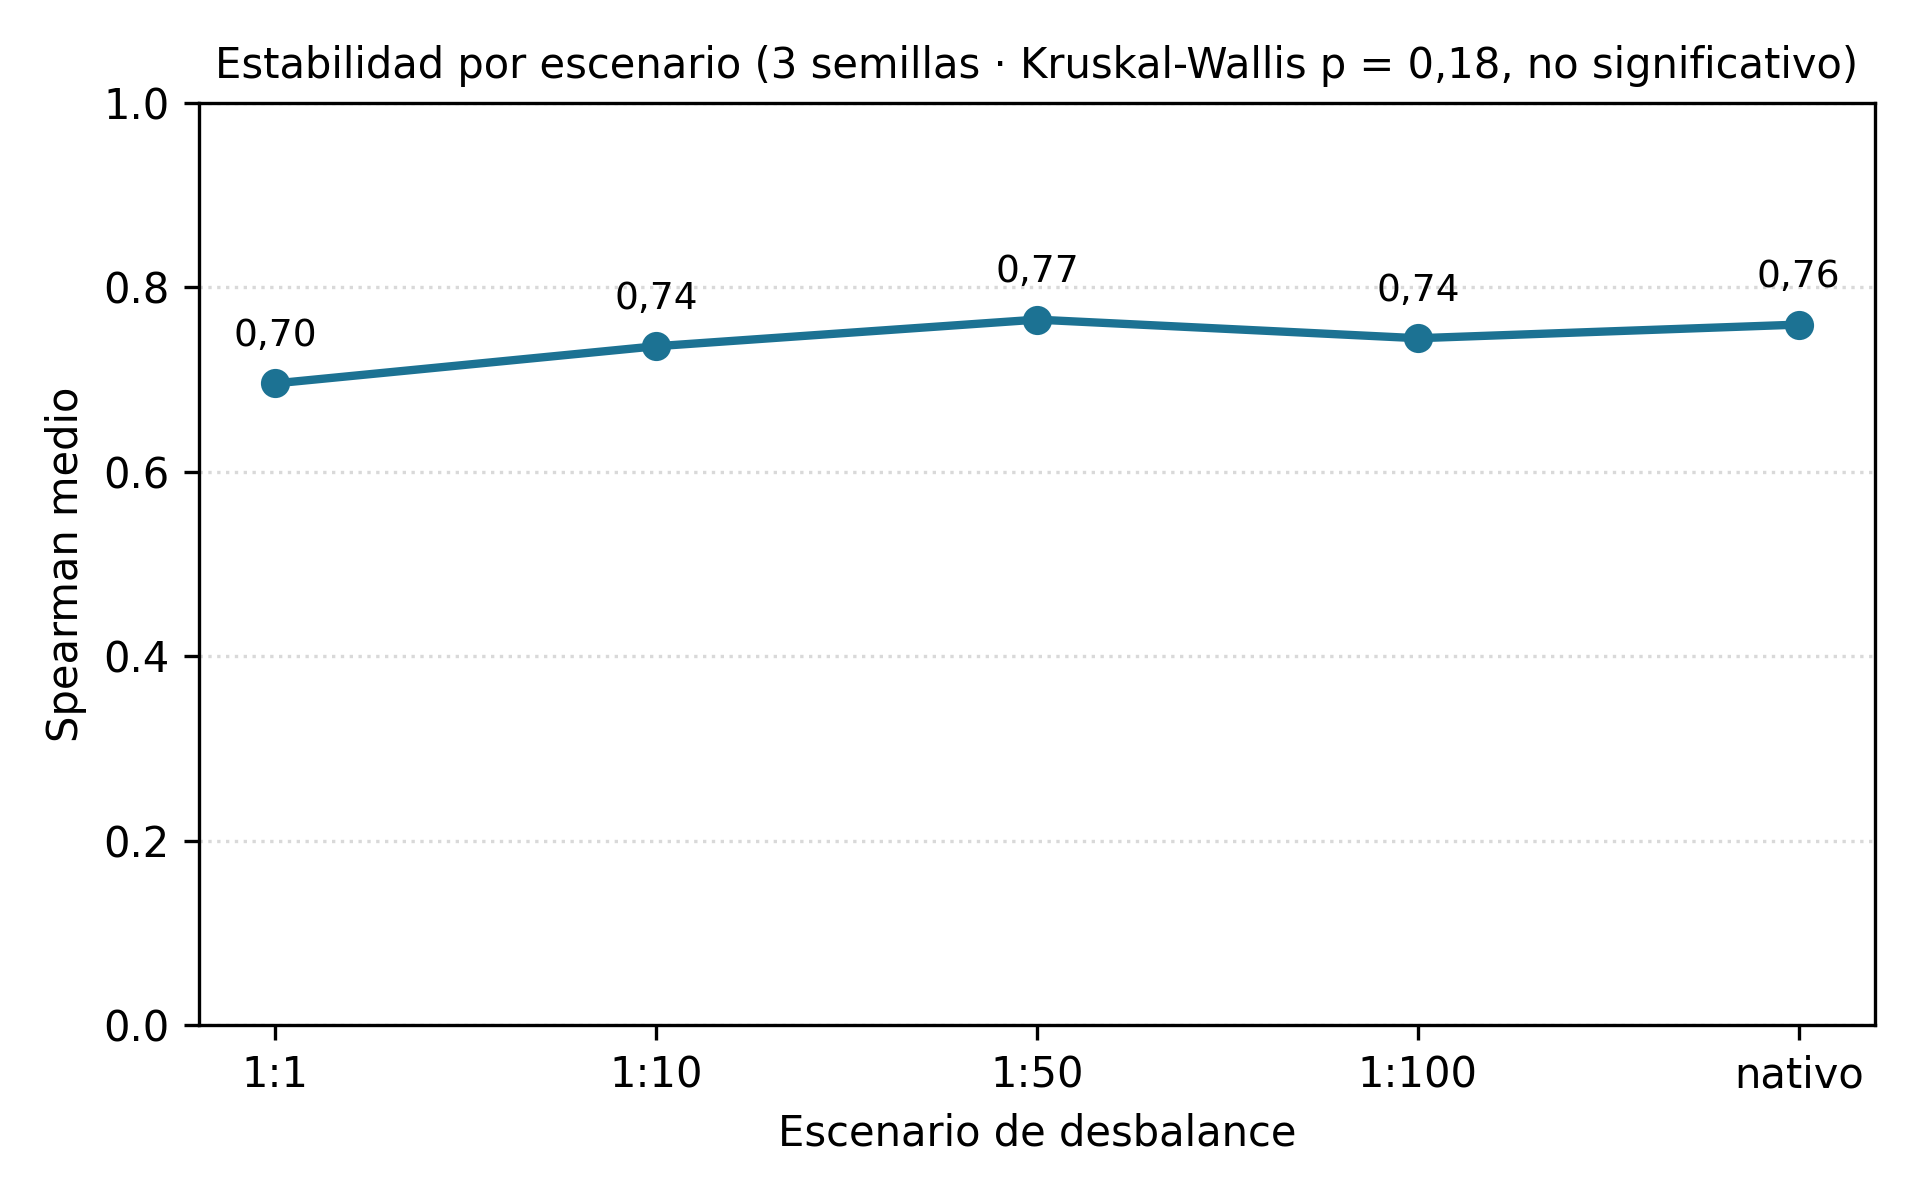
\includegraphics[width=0.8\textwidth]{chapter_4/images_ch4/estabilidad_escenario.png}
    \caption{Estabilidad de las explicaciones por escenario de desbalance sobre el subgrafo receptivo. El perfil es esencialmente plano, sin un pico de inestabilidad en el escenario 1:50 y con el valor más bajo en el escenario nativo, lo que invalida la interpretación previa de un deterioro localizado.}
    \label{fig:escenario}
\end{figure}

\begin{table}[htbp]
\centering
\renewcommand{\arraystretch}{1.3}
\begin{tabular}{lccccc}
\toprule
\textbf{Arquitectura} & 1:1 & 1:10 & 1:50 & 1:100 & nativo \\
\midrule
GraphSAGE & 0,715 & 0,748 & 0,761 & 0,697 & 0,751 \\
GAT & 0,750 & 0,811 & 0,798 & 0,765 & 0,785 \\
GCN & 0,697 & 0,760 & 0,787 & 0,757 & 0,793 \\
TAGCN & 0,622 & 0,626 & 0,703 & 0,752 & 0,704 \\
\midrule
\textbf{Media} & 0,696 & 0,736 & 0,765 & 0,745 & 0,760 \\
\bottomrule
\end{tabular}
\caption{Estabilidad de las explicaciones (correlación de Spearman de GNNExplainer) por arquitectura y escenario de desbalance sobre el subgrafo receptivo, promediada sobre las tres semillas de modelo. GCN y GAT encabezan la estabilidad de forma transversal a los escenarios, y la fila de medias muestra que el nivel de desbalance no ordena los resultados.}
\label{tab:elliptic-stab-scen}
\end{table}


La corrección obliga además a retractar el supuesto compromiso entre exactitud y estabilidad que la versión anterior reportaba con una correlación cercana a -0,20. Al haberse recomputado la estabilidad con una métrica corregida, aquella correlación deja de ser válida tal como se reportó y no puede sostenerse como un hallazgo del estudio. La lectura prudente es que el rendimiento en test colapsa de forma transversal en las cuatro arquitecturas, de modo que no existe una base sólida para afirmar una disyuntiva entre exactitud y estabilidad. Este episodio ilustra, además, un riesgo metodológico general en la evaluación de explicadores, el de que fallos silenciosos de cómputo o de medida se confundan con propiedades genuinas de las arquitecturas.

\section{Degeneración de PGExplainer en un Grafo Disperso}

Un resultado adicional del eje Elliptic concierne al comportamiento de PGExplainer sobre un grafo tan disperso. En este conjunto de datos, PGExplainer produce de forma casi universal una correlación de Spearman nula, un fenómeno de colapso de modo en el que el explicador asigna prácticamente la misma importancia a todas las aristas. La revisión de su implementación permitió corregir varios problemas, entre ellos reducir el tamaño de arista de 0,05 a 0,005 y ajustar la temperatura con un recorte para evitar desbordamientos numéricos, lo que estabilizó el entrenamiento del explicador. Aun así, cerca del noventa por ciento de los valores permanecen vacíos en Elliptic debido a la dispersión, de manera que la degeneración no se resuelve por completo en este dominio. Este resultado se reporta como un hallazgo metodológico y, como se verá en el Capítulo 5, contrasta de forma reveladora con el comportamiento del mismo explicador sobre un grafo denso.

La revisión de PGExplainer merece un comentario adicional por su valor metodológico. El colapso de modo observado, en el que el explicador asigna una importancia casi uniforme a todas las aristas, se manifiesta como una correlación de Spearman nula porque no existe un ranking de importancia que comparar entre ejecuciones. Las correcciones introducidas, que reducen el tamaño de arista y ajustan la temperatura del muestreo con un recorte numérico, atacan las causas de inestabilidad del entrenamiento del explicador, pero no pueden crear estructura donde el grafo no la ofrece. Por esta razón, aun con las correcciones, el explicador sigue produciendo una alta proporción de valores vacíos en Elliptic, lo que confirma que la limitación es del dato y no del ajuste del método.

Este resultado admite una lectura que trasciende el caso particular de PGExplainer. Un explicador que degenera sobre un conjunto de datos no es necesariamente un método deficiente, sino que puede estar reflejando una limitación estructural del grafo sobre el que opera. Distinguir entre ambas situaciones exige comparar el comportamiento del método en regímenes de densidad distintos, algo que un estudio de un solo conjunto de datos no permite. El eje sintético del capítulo siguiente proporciona precisamente ese contraste, y su resultado, que se anticipa aquí, invierte por completo el juicio sobre este explicador.

\section{Síntesis del Eje Elliptic}

El eje Elliptic deja tres conclusiones que enmarcan el resto de la tesis. La primera es que la dispersión extrema del grafo limita de manera estructural lo que puede medirse, hasta el punto de que el índice de Jaccard resulta trivial y la plausibilidad de las explicaciones no es evaluable en este dominio. La segunda es que el colapso de validación a test, causado por el desplazamiento temporal del dato, obliga a estudiar la estabilidad sobre validación y a declarar esta restricción con transparencia. La tercera es que la corrección sucesiva de un artefacto de memoria y de un defecto en la métrica de estabilidad disuelve la aparente ventaja de GraphSAGE y alinea el orden de estabilidad de Elliptic con el del grafo sintético, en el que GCN y GAT encabezan, de manera que la resiliencia explicativa no se invierte con la densidad sino que se manifiesta de forma concordante entre regímenes. Estas limitaciones, lejos de invalidar el estudio, motivan el eje sintético del Capítulo 5, concebido precisamente para medir aquello que el Elliptic Dataset no permite, la plausibilidad de las explicaciones frente a un \textit{ground-truth} conocido.
